\section{Diskussion}

\subsection{Kvalitet af sCT}


Vi har genereret en del flere sCT som ikke er blevet brugt i rekonstruktioner,  og de fleste er blevet af ret god kvalitet, som kan ses på figur~\ref{loocv_ct}. Omkring 20\% af sCT billederne har dog større problemer i selve hjernen.

\begin{figure}
   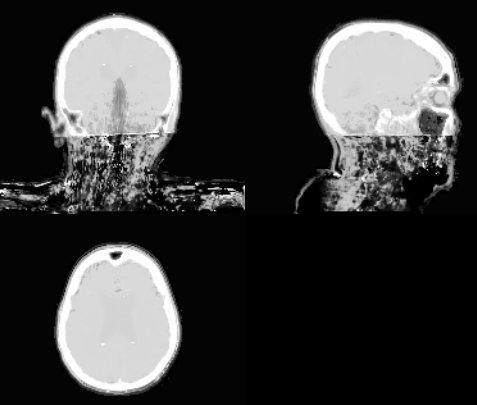
\includegraphics[width=\textwidth]{billeder/sct_problemer.png}
   \caption{sCT med problemer i hjernen. Der er mange punkter med både meget lave og meget høje værdier spredt rundt i selve hjernen.}
   \label{sct_problemer}
\end{figure}

På figur~\ref{sct_problemer} kan man se mange steder med lave værdier mellem knoglen og hjernen. Også inde i midten af hjernen er der problemer med både for høje og lave værdier. Vi er ikke klar over hvorfor nogen patienter bliver meget dårligere end de fleste andre, men Johansson et al. nævner at der kan være problemer med sampling mønstret for UTE sekvenserne.

På en del af billederne er det muligt at se ventriklerne, hvilket man ikke kan på CT billederne i samme grad.

Et væsentligt problem for sCT billederne ligger i at knoglerne bliver tykkere end på de rigtige CT billeder. Det kan ses på differens billederne på figure~\ref{col:loocv_ct_pat1_sub},~\ref{col:loocv_ct_pat1_sub},~\ref{col:loocv_ct_pat2_sub},~\ref{col:loocv_ct_pat3_sub},~\ref{col:loocv_ct_pat4_sub},~\ref{col:loocv_ct_pat5_sub}, da der en to lyse streger rundt om kraniet. Til gengæld ligger værdierne for sCT knoglerne i gennemsnit under værdierne i CT knoglerne, hvilket kan ses på farverne imellem figurene~\ref{col:loocv_ct_pat1_ct},~\ref{col:loocv_ct_pat2_ct},~\ref{col:loocv_ct_pat3_ct},~\ref{col:loocv_ct_pat4_ct},~\ref{col:loocv_ct_pat5_ct} og figurene~\ref{col:loocv_ct_pat1_sct},~\ref{col:loocv_ct_pat2_sct},~\ref{col:loocv_ct_pat3_sct},~\ref{col:loocv_ct_pat4_sct},~\ref{col:loocv_ct_pat5_sct}. Derfor ved vi ikke om det har en stor eller lille indflydelse på PET rekonstruktionen.

\begin{figure}
    \centering
    \begin{subfigure}[b]{0.3\textwidth}
        \caption{CT for patient 1.}
        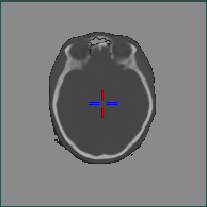
\includegraphics[width=0.75\textwidth]{colager/loocv_ct/loocv_010476_ct.png}
        \label{col:loocv_ct_pat1_ct}
    \end{subfigure}\hfill
    \begin{subfigure}[b]{0.3\textwidth}
        \caption{sCT.}
        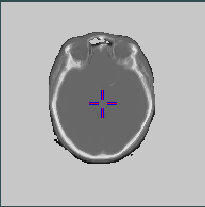
\includegraphics[width=0.75\textwidth]{colager/loocv_ct/loocv_010476_sct.png}
        \label{col:loocv_ct_pat1_sct}
    \end{subfigure}\hfill
    \begin{subfigure}[b]{0.3\textwidth}
        \caption{Differens.}
        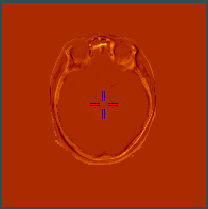
\includegraphics[width=0.75\textwidth]{colager/loocv_ct/loocv_010476_sub.png}
        \label{col:loocv_ct_pat1_sub}
    \end{subfigure}\\
    \begin{subfigure}[b]{0.3\textwidth}
        \caption{CT for patient 2.}
        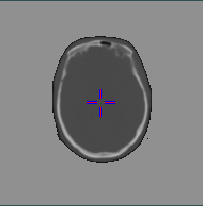
\includegraphics[width=0.75\textwidth]{colager/loocv_ct/loocv_010769_ct.png}
        \label{col:loocv_ct_pat2_ct}
    \end{subfigure}\hfill
    \begin{subfigure}[b]{0.3\textwidth}
        \caption{sCT.}
        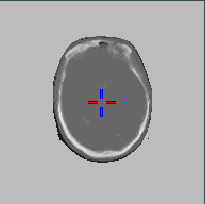
\includegraphics[width=0.75\textwidth]{colager/loocv_ct/loocv_010769_sct.png}
        \label{col:loocv_ct_pat2_sct}
    \end{subfigure}\hfill
    \begin{subfigure}[b]{0.3\textwidth}
        \caption{Differens.}
        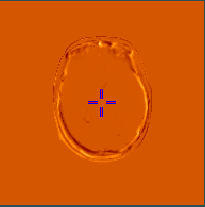
\includegraphics[width=0.75\textwidth]{colager/loocv_ct/loocv_010769_sub.png}
        \label{col:loocv_ct_pat2_sub}
    \end{subfigure}\\
    \begin{subfigure}[b]{0.3\textwidth}
        \caption{CT for patient 3.}
        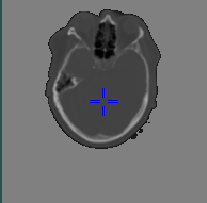
\includegraphics[width=0.75\textwidth]{colager/loocv_ct/loocv_010850_ct.png}
        \label{col:loocv_ct_pat3_ct}
    \end{subfigure}\hfill
    \begin{subfigure}[b]{0.3\textwidth}
        \caption{sCT.}
        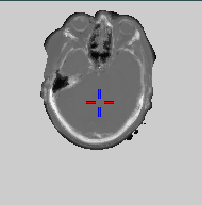
\includegraphics[width=0.75\textwidth]{colager/loocv_ct/loocv_010850_sct.png}
        \label{col:loocv_ct_pat3_sct}
    \end{subfigure}\hfill
    \begin{subfigure}[b]{0.3\textwidth}
        \caption{Differens.}
        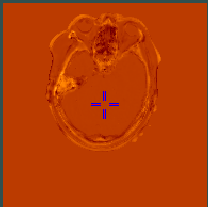
\includegraphics[width=0.75\textwidth]{colager/loocv_ct/loocv_010850_sub.png}
        \label{col:loocv_ct_pat3_sub}
    \end{subfigure}\\
    \begin{subfigure}[b]{0.3\textwidth}
        \caption{CT for patient 4.}
        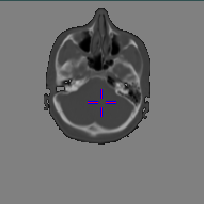
\includegraphics[width=0.75\textwidth]{colager/loocv_ct/loocv_010960_ct.png}
        \label{col:loocv_ct_pat4_ct}
    \end{subfigure}\hfill
    \begin{subfigure}[b]{0.3\textwidth}
        \caption{sCT.}
        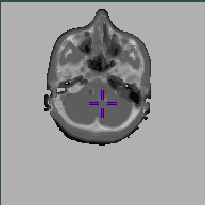
\includegraphics[width=0.75\textwidth]{colager/loocv_ct/loocv_010960_sct.png}
        \label{col:loocv_ct_pat4_sct}
    \end{subfigure}\hfill
    \begin{subfigure}[b]{0.3\textwidth}
        \caption{Differens.}
        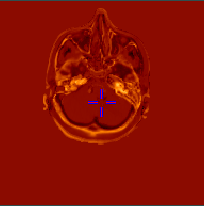
\includegraphics[width=0.75\textwidth]{colager/loocv_ct/loocv_010960_sub.png}
        \label{col:loocv_ct_pat4_sub}
    \end{subfigure}\\
    \begin{subfigure}[b]{0.3\textwidth}
        \caption{CT for patient 5.}
        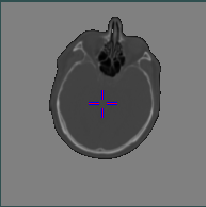
\includegraphics[width=0.75\textwidth]{colager/loocv_ct/loocv_011030_ct.png}
        \label{col:loocv_ct_pat5_ct}
    \end{subfigure}\hfill
    \begin{subfigure}[b]{0.3\textwidth}
        \caption{sCT.}
        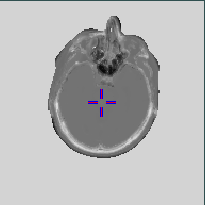
\includegraphics[width=0.75\textwidth]{colager/loocv_ct/loocv_011030_sct.png}
        \label{col:loocv_ct_pat5_sct}
    \end{subfigure}\hfill
    \begin{subfigure}[b]{0.3\textwidth}
        \caption{Differens.}
        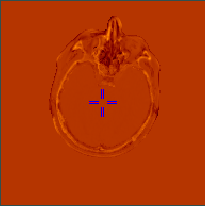
\includegraphics[width=0.75\textwidth]{colager/loocv_ct/loocv_011030_sub.png}
        \label{col:loocv_ct_pat5_sub}
    \end{subfigure}
    \caption{CT, sCT og differencen imellem dem for de fem patienter.}
    \label{col:loocv_ct}
\end{figure}

\subsection{Sammenligning med Johansson et al}


Som det ses på figur~\ref{fig:cumm_diff_loocv} er de fleste af vores sCT dårligere kvalitet i forhold til Johansson et al. Patient 1 følger nogenlunde samme kurve som Johansson et al. har fundet frem til. Ligeledes, hvis vi ser på figur~\ref{fig:loocv_j_h}, får vi samme features som Johansson et al. fremhæver.


Vi er ikke sikre på hvorfor vores de fleste af vores sCT er blevet dårligere. Vi tror det er en kombination af flere ting. 


For det første er vores masker ikke optimale, hvilket kan resultere i dårlige modeller. For det andet kan registreringen af sCT og CT ligge en smule forkert. Eftersom vi sammenligner på voxel niveau kræver det at registreringen er så tæt på perfekt som muligt, hvis alt er forskudt bare en enkelt voxel kan det gøre en stor forskel. For det tredje har de formentligt brugt patienter med bedre T2 billeder.


Dog mener vi ikke det har noget med algoritmen at gøre. Vi bruger EM, initialiseret med k-means, hvilket gerne skulle give det samme output hver gang. Da Johansson et al. bruger samme fremgangsmetode mener vi derfor problemet ligger i forbehandlingen af billederne.


Vi prøvede at træne med dobbelt så mange patienter, for at se om det gav bedre resultater, men det havde ikke nogen mærkbar effekt på sCT billederne.


\subsection{Billedformater}

I løbet af projektet har vi oplevet en del problemer med konverteringer
mellem filtyper. Vi benyttertre forskellige. Siemens scannerne producerer
Dicom billeder som vi arbejder med i Osirix, der er et medicinsk
billedbehandlisk program. Men det er et meget stort format, der ikke er
let at arbejde med. 

På Rigshospitalet er normen at konvertere til Minc, men vi havde planer,
om at bruge ITK, og Nifti var bedre understøttet i det. I sidste ende
endte vi med at registrere vores CT billeder i Minc, så vores billeder gik
igennem alle tre typer. 

Fra Dicom til Minc mister man en skalar, som man skal tage højde for, når
man konvertere tilbage. Ved konvertering fra Minc til Nifti, hvilket vi
kun gør med vores registrerede CT billeder, bliver de laveste værdier til
-1024, dem trækker vi endnu 1025 fra, så de kommer til at matche vores
laveste værdier.

\todo{Uddyb tab ved Dicom til Minc}

At konvertere til Dicom er ikke helt trivielt, så vi konverterer først til
Minc, hvor vi lægger 2048 til for at gøre op for det offset, der skete ved
den tidligere konvertering. 

Mange af disse problemer har vi opdaget så sent i processen, at vi ikke
har kunnet nå at tage hånd om dem. Den gennemsnitlige værdi i alle vores
Nifti billeder, som vi har trænet og testet på, har været for lav, og at
lægge en værdi til ved tilbagekonverteringen udbedrer det ikke, men ændrer
bare værdierne til samme størrelse, som i det målte CT.



